%\documentclass{sig-alternate}
\documentclass[twocolumn,10pt]{article}
\usepackage{times}

\usepackage{graphicx,url,color}
\usepackage[noend]{algpseudocode}
\usepackage{algorithm}
\usepackage{listings}
\usepackage{paralist}
\usepackage{amsmath}
%\usepackage{caption}yes
\usepackage[skip=0pt]{subcaption}
%\usepackage[tight]{subfigure}
\usepackage{eepic}
%\usepackage{dblfloatfix} % fix for bottom-placement of figure 
%\usepackage{perpage}
\usepackage{balance}
\usepackage{multicol}


\usepackage{caption}
\usepackage{subcaption}



\oddsidemargin 4.5pc
\evensidemargin 4.5pc
\advance\oddsidemargin by -1in  % Correct for LaTeX gratuitousness
\advance\evensidemargin by -1in % Correct for LaTeX gratuitousness
\marginparwidth 0pt             % Margin pars are not allowed.
\marginparsep 11pt              % Horizontal space between outer margin and
                                % marginal note

                                % Top of page:
\topmargin 4.5pc                % Nominal distance from top of page to top of
                                % box containing running head.
\advance\topmargin by -1in      % Correct for LaTeX gratuitousness
\headheight 0pt                 % Height of box containing running head.
\headsep 0pt                    % Space between running head and text.
                                % Bottom of page:
\footskip 30pt                  % Distance from baseline of box containing foot
                                % to baseline of last line of text.
\advance\topmargin by -37pt     % Leave 37pt above text for headers
\headheight 12pt                % Height of box containing running head.
\headsep 25pt                   % Space between running head and text.

\textheight 666pt       % 9 1/4 column height
\textwidth 42pc         % Width of text line.
                        % For two-column mode:
\columnsep 2pc          %    Space between columns
\columnseprule 0pt      %    Width of rule between columns.
\hfuzz 1pt              % Allow some variation in column width, otherwise it's
                        % too hard to typeset in narrow columns.
\newcommand{\ignore}[1]{}


\usepackage{subcaption}
\usepackage{microtype}

\bibliographystyle{abbrv}

\newcommand{\inred}[1]{{\color{red}{#1}}}
\newcommand{\inblue}[1]{{\color{blue}{#1}}}
\newcommand{\remove}[1]{}


% declaration of variables and foreach blocks
\algblock{Vars}{EndFor}
\algrenewtext{Vars}{variables}
\algrenewtext{EndVars}{}
\algblock{ForEach}{EndFor}
\algrenewtext{ForEach}{for each }

\begin{document}


\title{Fast Concurrent Data Sketches} 
%with Lightweight Synchronization}


\author{
Alexander Spiegelman\footnotemark[1] \ 
Edward Bortnikov\footnotemark[2]  \
Eshcar Hillel\footnotemark[2] \ 
Idit Keidar\footnotemark[1]\footnotemark[2] \ 
Lee Rhodes\footnotemark[2]\\ 
\footnotemark[1] Technion\ \ \footnotemark[2] Yahoo Research, Oath
}


\date{}


\maketitle


\begin{abstract}
Sketches are algorithms extracting information from a stream of data in a single pass. A query then generates approximate result with bounded error. Sketches are implemented as small efficient data structures using various randomization techniques. Despite the fact that they are designed to be used in big data systems for real time processing their current implementation is not thread-safe; each sketch object can be accessed only by a single thread at a time.
Our goal is to design  sketches that (1) allow queries to be processed while the sketch is being built; and (2) 
support parallel construction of the sketch via multiple threads.
The challenge is that a sketch update is not always atomic, and intermediate 
states of the sketch may be bogus, leading to gross estimation errors. 
For this reason, some applications that use sketches synchronize all access to them, which, is detrimental to performance (in our experiment, reducing throughput threefold). 
An approach with multiple threads, each summarizing a sub-stream followed by a union operator that merges all the sub-stream sketches
does not allow queries to be processed in real-time before the sketch is  merged.

We present a general approach for building concurrent sketches that
constantly reflect all data processed by multiple update threads, 
and serve queries at any time. We focus on concurrent implementations for the theta (count distinct) and quantiles sketches. 
Experiments show the algorithms' high performance and scalability in write-only and mixed read-write workloads.
\end{abstract}

\section{Introduction}

%\subsection{Motivation and goals}

% stream processing for RT analytics
Real-time analytics are becoming increasingly prevalent in many businesses. 
Examples include Yahoo's Flurry~\cite{flurry},  
%\footnote{\url{https://developer.yahoo.com/flurry/docs/analytics/}},
the technology behind Mobile Developer Analytics, and Digits Yahoo Corporate-Wide dashboard for monitoring KPIs and traffic trends%at different granularities
~\cite{digits},
%\footnote{\url{https://digits3.yahoo.com}},
as well as Google's F1~\cite{Shute2013}, which powers its AdWords
%\footnote{\url{https://www.google.com/adwords/}}
business.
Such systems need to process massive data streams and answer queries about them in real-time.
% examples
A common query, for example, is estimating the number of \emph{unique elements} in a long stream, which 
can be used to count how many different users access a particular web page or application. 
A second example is a \emph{quantiles} estimator, which can be used, for example, to  answer questions like  \emph{what percentage of user sessions end within one minute?} or \emph{what is the median session time?}

% Sketches
In order to serve such queries, analytics engines use 
\emph{data sketches}, or \emph{sketches} for short. A sketch is essentially 
a succinct summary of a long stream. 
Sketches are built in a single pass over the stream via sampling or by applying a filter 
that retains a small subset  of the stream elements. 
%They are designed to take up a small memory footprint, since analytics engines 
%often keep tens or hundreds of thousands and sometimes even millions of 
%sketches in memory~\cite{Druid}.
% Sketches are fast
Due to the massive scale of the incoming data,   library functions producing sketches
are optimized to be extremely fast, often digesting millions of stream elements per second~\cite{sketchesLibrary}. 

%For example, the $\Theta$ sketch in the Java Sketches Library \inred{add reference} 
%estimates the number of unique elements in a stream; it can process millions of stream 
%elements a second. 

 % Missing: r-w concurrency 
 Analytics engines need to answer real-time queries while  stream data continues to flow in.
 One way this is done 
today is by building sketches in epochs, and querying the sketch only after
 the epoch ends. An alternative approach is using locks to prevent concurrent access to a sketch.
 For example, in the Java Sketches Library~\cite{sketchesLibrary},  an 
attempt to query a sketch  while it is being updated  may encounter an inconsistent
intermediate state, leading to a gross estimation error. Therefore, applications like Druid~\cite{druid}
currently use sketches conservatively within a \emph{synchronized} block.
% and queries directed to a sketch must wait  for its construction to complete. 
Our first goal in this paper is to eliminate such waiting, and to allow queries to proceed 
concurrently with stream updates. 

% MIssing: w-w concurrency
In addition to the required concurrency among queries and updates,
it is also desirable to allow
concurrency among update threads in order to expedite the sketch building process on multi-core platforms. 
The common approach today is to build separate sketches from substreams, 
and then merge them via a dedicated union operation~\cite{multi-KMV}. 
In this approach, queries cannot be served before the final union completes. 
Our second goal is therefore to allow multiple threads to update a common, 
queryable sketch. The challenge is to do so without slowing down the update threads,
given that access to shared data requires  synchronization via costly memory fences 
and shared data updates can cause frequent invalidations in L1 caches, severely impacting performance. 
Figure~\ref{fig:lockBased} compares the throughput of two 
%  the
sequential sketch implementations given in DataSketch with
and without a lock. We see that 
the cost of acquiring a lock  is  high, since  sketches are
inherently fast structures.

\begin{figure}[t!]
    \centering
    \begin{subfigure}[t]{0.49\columnwidth}
        \centering
        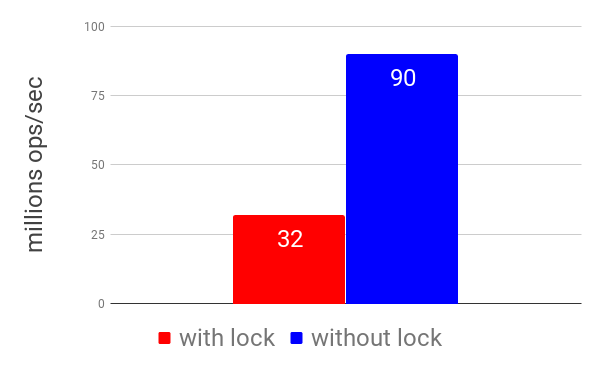
\includegraphics[width=1.6in]{images/seqTheta}
        \caption{Theta sketch}
        \label{fig:LockIsBadTheta}
    \end{subfigure}%
    ~ 
    \begin{subfigure}[t]{0.49\columnwidth}
        \centering
        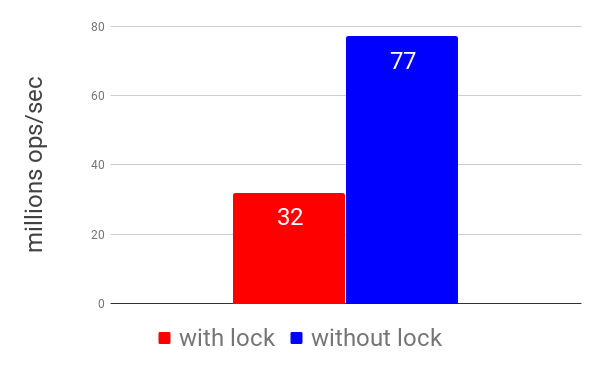
\includegraphics[width=1.6in]{images/seqQuantiles}
        \caption{Quantile sketch}
        \label{fig:LockIsBadQuantiles}
    \end{subfigure}
    \caption{Throughput of sequential sketch vs. lock-based sketch running a single write-only thread.}
    \label{fig:lockBased}
\end{figure}



% This paper
In this paper 
we present a general approach for building concurrent sketches that
constantly reflect all data processed by multiple update threads, 
and serve queries at any time. % during the stream processing. 
 % Basic idea for parallelizing
Our  approach employs multiple worker threads that buffer sketches of bounded-size substreams in thread-local memory, while a dedicated helper thread 
periodically \emph{propagates} these local buffers into a shared data structure via a union-like operation.
 Reducing data contention and the frequency of synchronization between the worker threads and the propagator is instrumental for achieving good performance. Queries are served from the shared data structure, and are carefully 
 designed to take its \emph{consistent snapshot} in case it is updated in parallel with them.

We implement our approach for two popular sketches in the Java Sketches Library -- Theta~\cite{Theta},
which estimates the number of unique elements in a stream, and quantiles~\cite{quantiles}.
%worst-case error an adversarial scheduler can induce, 
Experiments show the algorithms scales almost linearly: with 28 threads, update throughput is an order of magnitude greater than with a single threads, while the 
read throughput is 3 orders of magnitude greater than that of a lock-based implementation.  


 

\section{Sketches API and Correctness}
\label{sec:api}


% API 
A sketch $S$ supports three main API methods -- 
\begin{description}
\item[$S$.update($a_i$)] processes stream element $a_i$; and 
\item[$S$.query(arg)] returns the function estimated by the sketch, for example, the number of unique elements; 
 takes an optional argument, e.g., the requested quantile.
 \item[$S$.union($S'$)] merges sketches $S$ and $S'$ into $S$.
 % that is, if $S$ initially represents stream A and $S'$ 
 %represents stream $A'$, then after this call, $S$ represents the union of the two streams. 
 Sketches that support this operator are called \emph{mergeable}.
\end{description}

% Sequential specification
Today, sketches are used sequentially; the entire stream $A = a_1, a_2, \dots a_n$ is processed 
and only then the sketch is queried. $S$.query(arg) then returns an estimate of the desired function 
on the entire stream. 
Sketches use randomization and their accuracy is defined in one of two ways:
\begin{enumerate}
\item An \emph{unbiased} sketch provides an estimate  $\hat{e}$ whose expectation is the correct quantity $e$ 
(for example, the number of unique elements in the stream in a $\Theta$ sketch).  
\remove{
The \emph{Relative Standard Error (RSE)} is then derived from the variance $\sigma^2(\hat{e})$  of the estimate
as 
\[ \sqrt {\frac{\sigma^2(\hat{e})}{e^2}} \]
For example, a $\Theta$ sketch consisting of  $K$ samples provides an unbiased approximation $\hat{u}$ of the 
number $u$ of unique elements in the stream with an RSE of $1/\sqrt{K-1}$.
}
\item A \emph{probably approximately correct}'s  result  estimates the correct result
within some error bound $\epsilon$ with a failure probability bounded by some parameter $\delta$.  
%For example, a quantiles sketch approximates the $\phi$ quantile of a stream with  $n$ elements 
%by returning an element with rank between $(\phi-\epsilon)n$ and  $(\phi+\epsilon)n$ with 
%probability at least $1-\delta$.

\end{enumerate} 

% Relaxed semantics
 The correctness criterion for our concurrent sketches is a flavor of 
 \emph{relaxed consistency} due to Henzinger et al.~\cite{Henzinger2013}    
 specifically, a restricted form of their   \emph{out-of-order} relaxation 
 that allows operations to ``overtake'' some of the updates that precede them.  
 For example, a query may return a result that reflects all but a bounded number of the updates
 that precede it. It also allows bounded re-ordering of updates.
%While relaxed semantics were previously used for traditional data structures like stacks~\cite{Henzinger} and priority queues~\cite{alistarh}, 
We believe that relaxed semantics are a natural fit for data sketches
as they are inherently approximate and typically summarize streams that  arise from multiple real-world sources  
and are collected over a network with variable delays. Thus, even if the sketch ensures strict semantics, 
queries might miss some real-world events that occur before them.
%, which is not qualitatively different than the  relaxed sketch. Second, sketches are inherently approximate, even when they are strict. 
Relaxing their semantics therefore makes sense, as long as it does not excessively increase the expected error. 
% correctness roadmap: derandomize,  strong serializability, Adversary model,
With that, proving the concurrent sketches' correctness and analyzing the sketches' error bounds
are out of the scope of this paper.

\remove{ 

\noindent Note that step 3 is the only step that we are required
to prove.


TODO: figure?

TODO: Think about a general scheme that captures both our
algorithm and we can prove is strong linearizable.

\textbf{Comment: I do not know how to bound the error in the
worst case since r-relaxed runs change the summaries internal structure
and thus can potentially add more error than just missing k
values.}



\subsection{General implementation approach}
\label{sub:approach}

% Goals and challenges
Our goal is to build data sketches that (1) allow queries to be processed while the sketch is being built; and (2) 
support parallel construction of the sketch via multiple threads.
The challenge in achieving (1) is that a sketch update is not always atomic, and intermediate 
states of the sketch may be bogus, leading to gross estimation errors. 
For this reason, some applications that use sketches synchronize all access to them, which, as we show below, is detrimental to performance (in our experiment, reducing throughput threefold). 
The challenge with (2) is again, the need to support concurrent queries. 
Although data sketches are naturally amenable to parallel construction via separate threads (or processes) that each summarize a substream followed by a union operator that merges all the substream sketches, this approach 
does not allow queries to be processed in real-time before the sketch is  merged. 




%data structure
While sketches are usually not defined and treated as such, we
prefer to look on sketches as probabilistic append-only data
structures.
Every sketch has an API to append data item to the summary and
an API to read statistics on data items appended so far. 
In Section~\ref{sec:model} we formally define sketches
sequential specification, and a variation of a linearizabilty
property that takes the allowed error into account.
%a slightly weaker linearizabilty
%property that allows us to deal with infinite streams of data.
%
Now once we consider sketches as data structures with sequential
specifications, and we define how a sketch should behave when
accessed concurrently by many threads, we can talk about
concurrent sketches.

%The price of synchronization
However, in contrast to traditional concurrent data-structures,(
e.g., skiplists and B-trees) sketches' algorithms require very
little computation.
So, we should be very careful with the the cost we add
for synchronization. 
For example, as mentioned above, our measurements show that
adding even a single fence per operation in a sequential
execution decreases the throughput by a factor of 3.
Therefore, in order to get a scalable implementation we clearly
have to use as little synchronization as possible.

%Our approach - localirty
Our approach is strongly based on locality.
The common idea for all sketches is to make as much local work
as possible and use very light synchronization to merge it. 
We let threads process data items locally and only once in a
while we propagate their local state to a dedicated background
thread that merge local states with the shared one.
Thanks to the sketches semantics and structure we are able to do
it with a little extra memory cost and sometimes without
increasing the error at all.
Since sketches algorithms use randomized mechanisms to filter
data items, it is very nature to do it in parallel and sometimes
merge the results.
Note that by giving each thread to work locally and using a
dedicated thread for propagation, we also exploit better the
cache locality and pay less during fences. 

% \subsection{General Scheme}
% \label{sub:generalScheme}
% 
% 
% 
% 
% Given a sketch $sk$ with a sequential implementation $S$ such
% that every run of $S$ satisfies $sk$'s sequential specification,
% we give a general scheme to create a concurrent version of
% $S$ that satisfies \emph{r-perforated linearization}.
% First, extend $S$ to support concurrent reads, and denote this
% implementation by $S'$.
% Then, a generic structure that includes (1) a shared
% instance of $S'$; and (2) local data structures $L_1,.. L_n$
% that buffer operations to be added to $S'$.
% To satisfy \emph{r-perforated linearization} ensure that ($A_1$)
% all buffer contain no more than k operations together; and
% ($A_2$) the propagation from each $L_i$ to $S'$ is equivalent to
% running the sequence of operations masked by $L_i$ on $S'$.
% In the following sections we present two concurrent algorithms
% using the above structure and prove that they satisfy conditions
% $A_1$ and $A_2$.
% 
% TODO:
% 
% Axioms
% 
% figure
%  proof
% 
% 
}
\section{Theta Sketches}
\label{sec:theta}

Our first example is a $\Theta$ sketch implemented using  the 
\emph{K Minimum Values  (KMV)} algorithm~\cite{KMV}, 
which estimates the number of unique items in a data stream. 
We first overview the sequential  sketch in Section~\ref{ssec:theta-overview}, 
and then explain how we parallelize it in Section~\ref{ssec:concurrent-theta}.
Section~\ref{ssec:theta-analysis} analyzes the algorithm's correctness and error bounds.

\subsection{Overview}
\label{ssec:theta-overview}


A $\Theta$ sketch maintains a set of samples and a parameter $\Theta$
that determines which elements are added to the sample set. 
It uses a random hash function whose outputs are uniformly distributed
in the range $[0,1]$, and $\Theta$ is always in the same range.  
Every incoming data stream element is first hashed, and then the hash is compared to $\Theta$. 
In case it is smaller, the value is added to the sample set.  Otherwise, it is ignored. 

Because the hash outputs are uniformly distributed, an expected
portion $\Theta$ of them are smaller than $\Theta$ and hence included in the sample. 
Therefore, we can estimate the number of unique data items in the stream by
simply dividing the number of (unique) stored samples by $\Theta$.
The error depends on the size of the sample set -- with $K$ samples, 
the  >
Note that 
this analysis assumes that the random hash function is drawn independently of the stream values.

 $\Theta$ sketches keep constant-size sample sets, independently of the stream size. 
 To this end, they need to adjust $\Theta$ on-the-fly, and prune elements of 
 the sample set whose hashes are smaller than the new $\Theta$.
%There are a number of approaches to do that. 
A straightforward KMV solution keeps a sample of size $K$ 
holding the  values with the $K$ smallest hashes seen so far. 
In this case $\Theta$ is $1$ during the first $K$ updates, and 
subsequently it is the hash of the largest sample in the set.
Once the sample set is full,
every update that inserts  a new element also removes the largest
element in the set and updates $\Theta$ accordingly. 
This can be implemented efficiently by keeping the samples in  a min-heap. 
A nice property of this KMV variant is that it is \emph{order agnostic}, i.e., produces 
identical results for streams that consist of the same elements albeit in a different order.

\inblue{ [[Let's try to replace quickselect by the straightforward variant in the experiments and remove this discussion. ]]
The slightly optimized \emph{quickselect} variant of KMV keeps samples 
in a hashmap, and  allows the sample size to vary between $K$ and $2K$
as illustrated in  Figure~\ref{fig:thetaSampling}.
Insertions are quicker as long as the hash does not overflow, and once
it does (i.e., includes $2K$ samples), the algorithm uses quickselect to 
find the $K^{th}$ smallest value and deletes all bigger values. 
This variant is not order agnostic, because the order in which elements appear can impact how many 
elements end up being sampled.
Note that since typically, $K \ll n$, the vast majority of hashes are larger than 
$\Theta$,  and so most update operations complete without updating the sample set. 
Therefore, the impact of this optimization is not dramatic. 
} 

\begin{figure}[H]
    \centering
    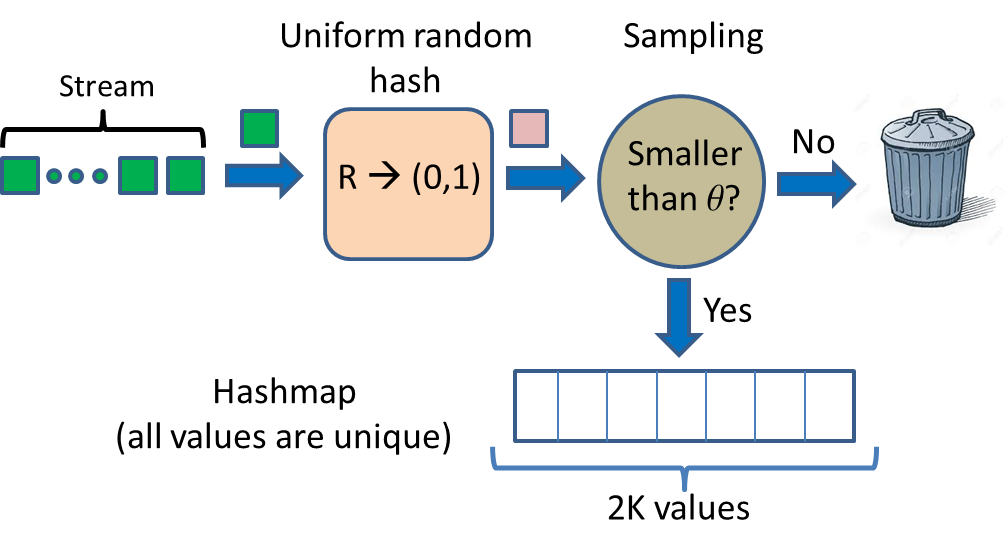
\includegraphics[width=2.5in]{images/thetaSampling.png}
    \caption{Sampling in quickselect KMV algorithm. \inred{I have many issues with this picture: (1) Fonts are too small. 
    (2) What is the R in the hash box? Please remove. 
    (3) The hashmap has 2K entries (not lower case k, not values). (4) Ifs in flowcharts are diamonds, not circles.
    (5) There is a missing diamond ``hash full?'' with pruning of the map and update of $\Theta$ in case of yes.
    Of course all this is only relevant if we decide to keep this algorithm.}}
    \label{fig:thetaSampling}
\end{figure}





\subsection{Concurrent algorithm}
\label{ssec:concurrent-theta}

%As mentioned in Section~\ref{sub:concurency}, 
Our concurrent implementation -- given in  Algorithm~\ref{alg:concurrent-theta} 
and illustrated in Figure~\ref{fig:concurrentTheta} --  
uses multiple threads to process incoming stream elements; 
it services queries at any time during the sketch's construction. 
%Since the only thing threads need to know in order to sample stream elements is
%the value of $\Theta$, they can do so locally in parallel, 
Update threads sample stream elements in parallel into local buffers, 
while a background thread periodically propagates the sampled values to a shared sketch
consisting of sampleSet and $\Theta$. 


\begin{algorithm}[tb]
\small
\begin{multicols}{2}
\begin{algorithmic}[1]

%\State {\bf Sketch variables:}
\Vars
\State   sampleSet, init $\emptyset$ \Comment global samples
\State  $\Theta$, init $1$			\Comment global threshold
\State {\tt atomic} est, init $0$ \Comment estimated \# uniques
\State $h$, init random uniform hash function 
\Statex
\ForEach{update thread $t_i$} 
	\State \emph{buf$_i$}, init $\emptyset$ \Comment local sample set
	\State \emph{aux$_i$}, init $[ ]$ \Comment auxiliary array
	\State $\Theta_i$, init $1$ 	\Comment local threshold
	\State {\tt atomic} $P_i$, init $1$ \Comment for synchronization
\EndFor
\EndFor

\Statex
\Procedure{query}{}
\State return est \label{l:query}
\EndProcedure
%\Statex

\Procedure{update$_i$}{val}
\If{$h$(val) $< \Theta_i$} 
	add val to \emph{buf$_i$} \label{l:local-sample}
\EndIf
\If{$|$\emph{buf$_i$}$| > b$} \Comment propagate
	\State wait until $P_i >0$ \label{l:wait}
	\State $\Theta_i \leftarrow P_i$ \label{l:adopt}
	\State \emph{aux$_i$}  $\leftarrow$ sort by $h$ $\{ e \in \mathit{buf_i} | h(e) <\Theta_i \}$
		\label{l:sort}
	\State $P_i \leftarrow 0$ 		\label{l:signal}
	\State \emph{buf$_i$}$ \leftarrow \emptyset$  \label{l:clean} 

\EndIf  
\EndProcedure

\Procedure{propagator}{}
\While {true}
\ForAll{update thread $t_i$ s.t. $P_i =0$} 
		\State  update sampleSet and $\Theta$ with \emph{aux$_i$} \label{l:aux}
		\State est $\leftarrow |$sampleSet$|/ \Theta$ \label{l:update-est}
		\State $P_i \leftarrow \Theta$  \label{l:theta}
\EndFor
\EndWhile
\EndProcedure

\end{algorithmic}
\end{multicols}
\caption{Concurrent $\Theta$ sketch algorithm.}
\label{alg:concurrent-theta}
\end{algorithm}

The key to achieving efficiency is exploiting locality and minimizing synchronization.
Every worker thread $t_i$ samples stream elements into a local bounded buffer 
\emph{buf$_i$} of size $b$ (line~\ref{l:local-sample}). 
To avoid frequent cache invalidations, $t_i$ uses a periodically refreshed
local copy $\Theta_i$ of $\Theta$. 
Because the global  $\Theta$ is monotonically decreasing, periodically copying it
into local copies maintains the invariant $\Theta_i \geq \Theta$.
Thus, while threads may over-sample, they never fail to sample elements that need 
to be included in the shared sketch. 
%Initially, all buffers are empty and all local $\Theta_i$s are $1$. 

When the buffer of a thread $t_1$ becomes full, $t_1$ sorts it
into an auxiliary array \emph{aux$_i$} and signals to the propagator  to union
it with the shared sketch (lines~\ref{l:sort}--\ref{l:signal}).
In the meantime, $t_1$ proceeds to re-fill its buffer with new samples.
The propagation  (line~\ref{l:aux}), in turn,  is highly optimized, as it merges a sorted array of 
values into the sampleSet, and can stop merging upon encountering 
an element whose hash is bigger than the global $\Theta$.

Update thread $t_i$ synchronizes with the propagator using a 
single \emph{atomic} variable $P_i$, which it sets to zero 
to signal to the propagator that the auxiliary array is ready.  
Because $P_i$ is  atomic, the Java memory model
guarantees that $t_i$'s auxiliary array is visible to
the background thread when $P_i$'s update is.
This is  an expensive operation (involving a memory fence),  
but we do it only once per $b$ items retained in the sample.

Before propagating its buffer, $t_i$ waits
until $P_i > 0$  (line~\ref{l:wait}); 
this indicates that the propagation of the previous \emph{aux}$_i$
 has completed, and  \emph{aux}$_i$ may
be reused. Thus, we  ensure that the sketch uses bounded space.
%
When the background thread completes the propagation, 
it piggybacks the global $\Theta$, which only it updates, on $P_i$  (line~\ref{l:theta}), 
and $t_i$ adopts it  (line~\ref{l:adopt}). Thus, update threads   learn $\Theta$ at no
additional synchronization cost. 

In order to support  fast concurrent reads, the shared sketch
maintains an atomic variable est, estimating the number of
 unique items seen so far by the propagator.
The background thread updates this variable after each propagation.
Again, because est is atomic, updating it involves a costly memory fence, which we amortize by performing it once per $b$ updates. 

For the $S$.union($S'$) operation (omitted from the code), 
we assume $S'$ is not undergoing any updates. 
The propagator thread puts its normal tasks on hold, 
 adopts the smaller $\Theta$ of the two sketches, merges their sampleSets while filtering elements according to the new $\Theta$, updates est, and resumes its 
 propagation tasks. Other operations (query and update) continue undisturbed.


\begin{figure}[H]
    \centering
    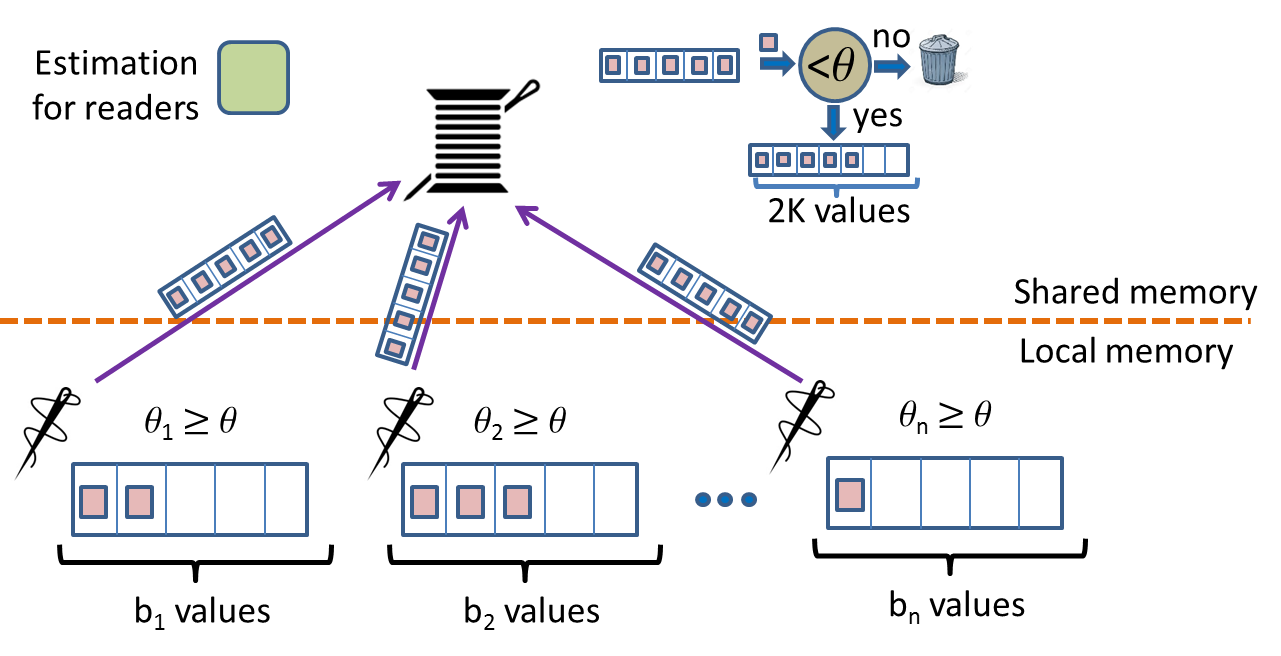
\includegraphics[width=4in]{images/thetaConcurrent.png}
    \caption{Concurrent $\Theta$ sketch architecture.
    \inred{Some requests for changes in the figure: 
    (1) Change $b_1$, $b_2$, and $b_3$ to $b$. 
    (2) Label the buffers as \emph{buf}$_1$ and \emph{aux}$_1$ etc. 
    (3) Write sort on one of the purple arrows. 
    (4) Replace 2K values with sampleSet.
    (5) remove the extra buffer on top, the aux buffered are merged directly into sampleSet. 
    (6) label the top thread as propagator.
    (7) Show a reader thread reading the estimate.
    (8) The classification of shared versus local memory is wrong. $\Theta$ and sampleSet are private
    	variables of the propagator.
    }}
    \label{fig:concurrentTheta}
\end{figure}

\subsection{Analysis}
\label{ssec:theta-analysis}

As explained above, we model the source of randomness used in the choice of $h$ as externally provided and the algorithm as  deterministic. We denote by $A^D_s$ the histories  of the deterministic sequential algorithm  (described in Section~\ref{ssec:theta-overview}) and by $A^r_s$ its $r$-relaxation. We denote by $A_c$ 
our (deterministic) concurrent algorithm (Algorithm~\ref{alg:concurrent-theta}).
%Section~\ref{ssec:concurrent-theta}).

When  $A_c$  uses $N$ update threads, its relaxation is $r=2Nb$. 
We first show that $A_c$  is strongly linearizable with respect to the relaxed specification $A^{2Nb}_s$,  and then analyze the error  of  $A^{2Nb}_s$.

\subsubsection{Strong linearizability wrt relaxed semantics}

For simplicity, we assume that lines  \ref{l:aux}--\ref{l:update-est} are executed atomically; 
in practice this assumption does not have any implications because $\Theta$ and sampleSet 
are private variables accessed only by the propagator.  

To prove correctness, we first show the following invariant about the samples maintained by 
our algorithm when using $N$ update threads.
\begin{invariant}[Sampling]
Consider a finite execution $\sigma$ of  $A_c$ and an update(v) that returns in $\sigma$. 
Then  at the end of $\sigma$,  if $h(v) < \Theta$ then 
$v\in \bigcup_{i=1}^N (\mathit{buf_i} \cup \mathit{aux_i}) \; \cup$ sampleSet.
\label{invariant:sampling}
\end{invariant}

\begin{proof}
The proof is by induction on the length of $\sigma$. The base for the empty execution is immediate. 
Now consider execution steps that can change the invariant.
First, consider an update that does not propagate \emph{buf$_i$}. 
Because each thread's $\Theta_i \le \Theta$ and a new update(v)  is sampled into \emph{buf$_i$} if 
$h(v) < \Theta_i$, the invariant is preserved.

Next, consider the propagation. 
In line~\ref{l:sort},  all elements of  \emph{buf$_i$}
whose hash value still exceeds $\Theta_i$ are inserted into \emph{aux$_i$} 
so clearing \emph{buf$_i$} in line~\ref{l:clean} preserves the invariant. 
It remains to show that when  \emph{aux$_i$} is overwritten in line~\ref{l:sort},
 all relevant entries from it have been propagated to  sampleSet (in line~\ref{l:aux}).
This is ensured by the atomic variable $P_i$, as follows:
(1) elements are added to \emph{aux$_i$} (line~\ref{l:sort}) only when $P_i >0$ while 
 the auxiliary thread propagates \emph{aux$_i$} into sampleSet according to $\Theta$ only when $P_i =0$,
 so \emph{aux$_i$} is never accessed concurrently by more than one thread;
(2) $P_i$ does not change from zero to non-zero unless  \emph{aux$_i$} has been propagated into sampleSet,
and is not overwritten by the update unless it changes from zero to non-zero. 
Finally, note that $\Theta$ is monotonically decreasing and previously sampled elements are removed from sampleSet only if their hashes exceed the new $\Theta$, again, preserving the invariant.
\end{proof}

Our strong linearizability proof uses two mappings,
$f$ and $g$,  from executions of $A_c$ to sequential executions. 
%
For an execution $\sigma$ of $A_c$,  $f(\sigma)$ is the sequential execution of $A_s$
consisting of  
operations invoked in $\sigma$,  ordered according to their invocation times. 
% when they execute their first step (line~\ref{l:query} for a query and~\ref{l:local-sample} for an update).
By definition, $f(\sigma)$ preserves the real-time order of $\sigma$ and $f$  is prefix-preserving.
To prove strong linearizability, it remains to show that $f(\sigma) \in A^{2Nb}_s$.

We define our second mapping, $g$, 
by ordering operations according to  \emph{visibility points} defined as follows: 
\begin{itemize}
\item
Visibility points of queries are their execution steps    (line~\ref{l:query}). 
%same as their linearization points. 
\item
For an update$_i$($v$) in $\sigma$, 
if $v$ is not added to \emph{buf$_i$} in line~\ref{l:local-sample}, then this point is its visibility point. 
%(as well as its linearization point). 
\item
Otherwise, consider an update$_i(v)$ that inserts $v$ into \emph{buf$_i$}, and  
let $t$ be the next time in $\sigma$ when thread $i$ propagates \emph{buf$_i$} into \emph{aux$_i$}
(i.e., executes line~\ref{l:sort}). The update's visibility point is 
the update of est (line~\ref{l:update-est}) that follows
the first propagation of \emph{aux}$_i$ into sampleSet (lines \ref{l:aux}--\ref{l:update-est})
after time $t$. 
\end{itemize}
 Note that in the latter case, 
the visibility point may occur after the update returns, and so $g$ does not 
necessarily preserve real-time order.

To complete the proof, we will show that for every execution $\sigma$ of $A_c$:
(1) ${\cal H}(g(\sigma)) \in A^D_s$, and 
(2)  ${\cal H}(f(\sigma))$ is a $2Nb$-relaxation of ${\cal H}(g(\sigma))$.  
Together, this will imply that ${\cal H}(f(\sigma)) \in A^{2Nb}_s$, as needed.  
%
To prove (1), we show the following invariant by induction on steps of  $\sigma$:

 \begin{invariant} 
 The values of $\Theta$, sampleSet, and est at the end of $\sigma$ are equal to the sequential sketch's 
  $\Theta$, sampleSet, and estimate at the end of $g(\sigma)$. 
  \label{inv:theta-est}
 \end{invariant} 

\begin{proof}
 The base is immediate because the variables are initialized the same way and the estimate is initially zero.
%Notice that the propagator is the only thread that updates $\Theta$, sampleSet, and est. 
Assume the invariant holds, and consider a new update$_i$($v$) operation. If $v$ is not retained 
in the sample according to $\Theta_i$, the update occurs in $g(\sigma)$. Note that in this case, 
$v$ would not have been sampled by the sequential sketch  
according to $\Theta$, which is $\le \Theta_i$, hence in both $\sigma$ and $g(\sigma)$ the variables are unchanged.
If the sample is retained, then line~\ref{l:local-sample} does not affect $\Theta$, sampleSet, or est,
and the update does not occur in $g(\sigma)$ yet, so again, the variables are unchanged in both.

Once \emph{aux$_i$} has been propagated (lines \ref{l:aux}--\ref{l:theta} occurred), 
 \emph{aux$_i$} may be overwritten, and by Invariant~\ref{invariant:sampling}, all the update$_i(v)$ operations 
reflected therein are included in sampleSet. Note that when they are propagated to sampleSet, they affect 
 $\Theta$, sampleSet, and est exactly like updates in the sequential sketch affect $\Theta$, sampleSet, and 
 the sketch's estimate. 
 Indeed, all updates that affected \emph{aux$_i$} since the last propagation are 
included in $g(\sigma)$ at this time (as it is their visibility point), and so the invariant is preserved. 
\end{proof}

Queries take effect instantaneously, and since est is  atomic, they return its up-to-date value in $\sigma$. 
In $g(\sigma)$, they return the sketch's estimate, which by Invariant~\ref{inv:theta-est} is the same.
Thus, ${\cal H}(g(\sigma))$ is a history of the sequential sketch, proving (1). 

To prove (2), observe first that since an operation's invocation is always at or before its 
visibility point, $g(\sigma)$ includes a subset of the operations in $f(\sigma)$. 
It remains to show  that every operation invocation in $g(\sigma)$ is preceded by all 
but at most $2Nb$  of the invocations that precede the same operation in $f(\sigma)$. 
To prove this, we show that for every prefix $\sigma'$ of $\sigma$, $g(\sigma')$ includes all 
but at most $2Nb$  of the invocations in $f(\sigma')$.
Observe that 
every operation in $f(\sigma')$ that is not included in $g(\sigma')$ is update$_i$($v$) such that $v$
was  retained in \emph{buf$_i$} and did not yet propagate to sampleSet at the end of $\sigma'$. 
In this case, by Invariant~\ref{invariant:sampling}, 
the update is either still in  \emph{buf$_i$} or in  \emph{aux$_i$}, each of which 
includes at most $b$ samples, and since there are $N$ update threads, there are at most $2Nb$ 
such values, as needed. 


We have proven the following:

\begin{lemma}%[Strong linearizability] 
$A_c$  with $N$ update threads is strongly linearizable wrt $A^{2Nb}_s$.
\label{lemma:theta-strong}
\end{lemma}

\subsubsection{Error bounds}

We analyze the error introduced by an $r$-relaxation $A^r_s$ of the $\Theta$ sketch.
Given Lemma~\ref{lemma:theta-strong} above, the concurrent sketch's error is bounded
by the relaxation's error bound for $r=2Nb$.  

Consider first a weak adversary, which chooses up to $r$ updates to hide from every query in advance,
before the oracle's coin flips. In this case, the adversary cannot bias the estimate computed
over unhidden updates. That is, it cannot select updates that are ``unlucky'' for the sketch, inducing 
a higher error, and hide others that induce a lower error. 
Thus, each query obtains an estimate of the number of unique elements
in some substream that includes all but at most $r$ of the stream elements, with the same error bound of the 
unrelaxed sketch (i.e., with an RSE of $1/\sqrt{K-1}$~\cite{KMV}). 
The adversary thus maximizes the error of the relaxed sketch by hiding as many unique elements as possible,
which is at most $r$. 
We get the following:
\begin{claim}
For a stream with $u$ unique elements, the expected estimate of an $r$-relaxation $A^r_s$ of the $\Theta$ sketch
with sample size $K$ under a weak adversary is between $u-r$ and $u$, and its  RSE is $1/\sqrt{K-1}$. 
\end{claim}

Next, consider a strong adversary. 
\inblue{In this case we should be able to analyze only the unoptimized version, with a min-heap not quickselect. It will require opening the box and looking at the algorithm and its analysis.}
Recall that at any point in the execution of the sequential sketch, $\Theta$ is the value with the $K^{th}$ smallest 
hash in updates so far, and sampleSet the $K$ smallest-hash elements.  
% Since $h$'s output is uniformly distributed in $[0,1]$, the expected size of $\Theta$ is 
  \inred{To Do!}

% TODO: Think more about the bound on the worst case error\ldots 

\section{Quantiles Sketch}
\label{sec:quantiles}


Given a stream $A$ of items from an ordered domain, for every
$0< \phi < 1$, $\phi$-quantile of $A$ is an item with rank 
$\lfloor \phi |A| \rfloor$, where the rank of item $i$ is the
number of elements in $A$ smaller than $i$.
An $\epsilon$-approximate ~$\phi$-quantile is an element
with rank between $ (\phi-\epsilon) |A|$ and $ (\phi +
\epsilon) |A|$.
For every stream $A$, error $\epsilon$, and probability $\delta$,
a quantiles sketch algorithm produces a summary of $A$, which
supports $\epsilon$-approximate ~$\phi$-quantile queries for
every $0< \phi < 1$ namely, returning an element with rank between $(\phi-\epsilon)n$ and  $(\phi+\epsilon)n$ with probability
at least $1 - \delta$.

\subsection{Overview}
As in the $\Theta$ sketch, there
is a tradeoff between the summaries' space cost and query accuracy,
which has been  studied in the past.
In this work we build on top of an algorithm presented
in~\cite{}, whose storage cost grows logarithmically with the
input stream size.
Given a stream $A$, the storage cost of the algorithm is
$k 2^{log(\lfloor |A|/k \rfloor)}$, where $k = O((1/\epsilon)
\sqrt{log(1/\epsilon \delta)}$.
The main idea is to 
\emph{merge} two sets, $S_1$ and $S_2$, consisting of $k$ items each, to a
single set $S$ of $k$ items.  This is done by first taking the sorted union of the sets, and  
then, with equal probability, retaining either the even or the odd
items in the sorted order. 
This process is called \emph{zip}.


The algorithm maintains $\lfloor log(|A|/k) \rfloor$ weighted
levels, where each level is an array of size $k$ that either contains $k$ ordered
items or is \emph{invalid} (see Figure~\ref{fig:quantilesMerge}).
The weight of level $i$ is $2^{i-1}$.
In addition, the algorithm uses a
\emph{bitPattern} variable that indicates which levels are valid,
and a \emph{base Buffer} of size $2k$, which is filled with items
from the stream.
Every time the baseBuffer is full, it is propagated (in place) to
the levels arrays in the following way:
First find using the bitPattern the first invalid level in
the levels array, 
call it the \emph{target} level. At the end of
the propagation this level becomes valid, while all the
level beneath it become invalid.
Next, sort and zip the base buffer (with equal probability,
pick either the even or the odd items in the sorted order) into
the target level.
Repeat the following process from level $i=1$ to the
last level that precedes the target level:
Mergesort level $i$ with what is currently stored in the target
level into the base buffer, and then zip the base buffer into the
target level.
Finally, update the bitPattern to indicate that the target
level is now valid while all the levels beneath it are not.

The weight of level $i+1$ is twice the weight of level
$i$ because it was zipped one more time, and thus it
``represents'' twice of the number of items ``represented'' in
level $i$.
This is important for quantiles accuracy.
In order to get a quantile we first have to build an
\emph{auxiliary} object that contains two arrays: 
(1) a sorted array of items, \emph{Iarr}, which 
contains all the items from all the valid levels, and (2) an
array of weights, called \emph{Warr}, that maps every item in
Iarr to its weight.
Then, to get the $\phi$-quantile, we %of a stream $A$
find the first index $ind$ in $Warr$ such that the
sum of all weights in $Warr$ till index $ind$ is $\lfloor \phi |A|
\rfloor$, and return $Iarr[ind]$. The algorithm is illustrated in
Figure~\ref{fig:quantilesMerge}.
%Since it is not the focus of our paper we omit the error analysis
%of the algorithm, and refer the interested reader to~\cite{} for
%the proof and more details.

\begin{figure}[tb]
    \centering
    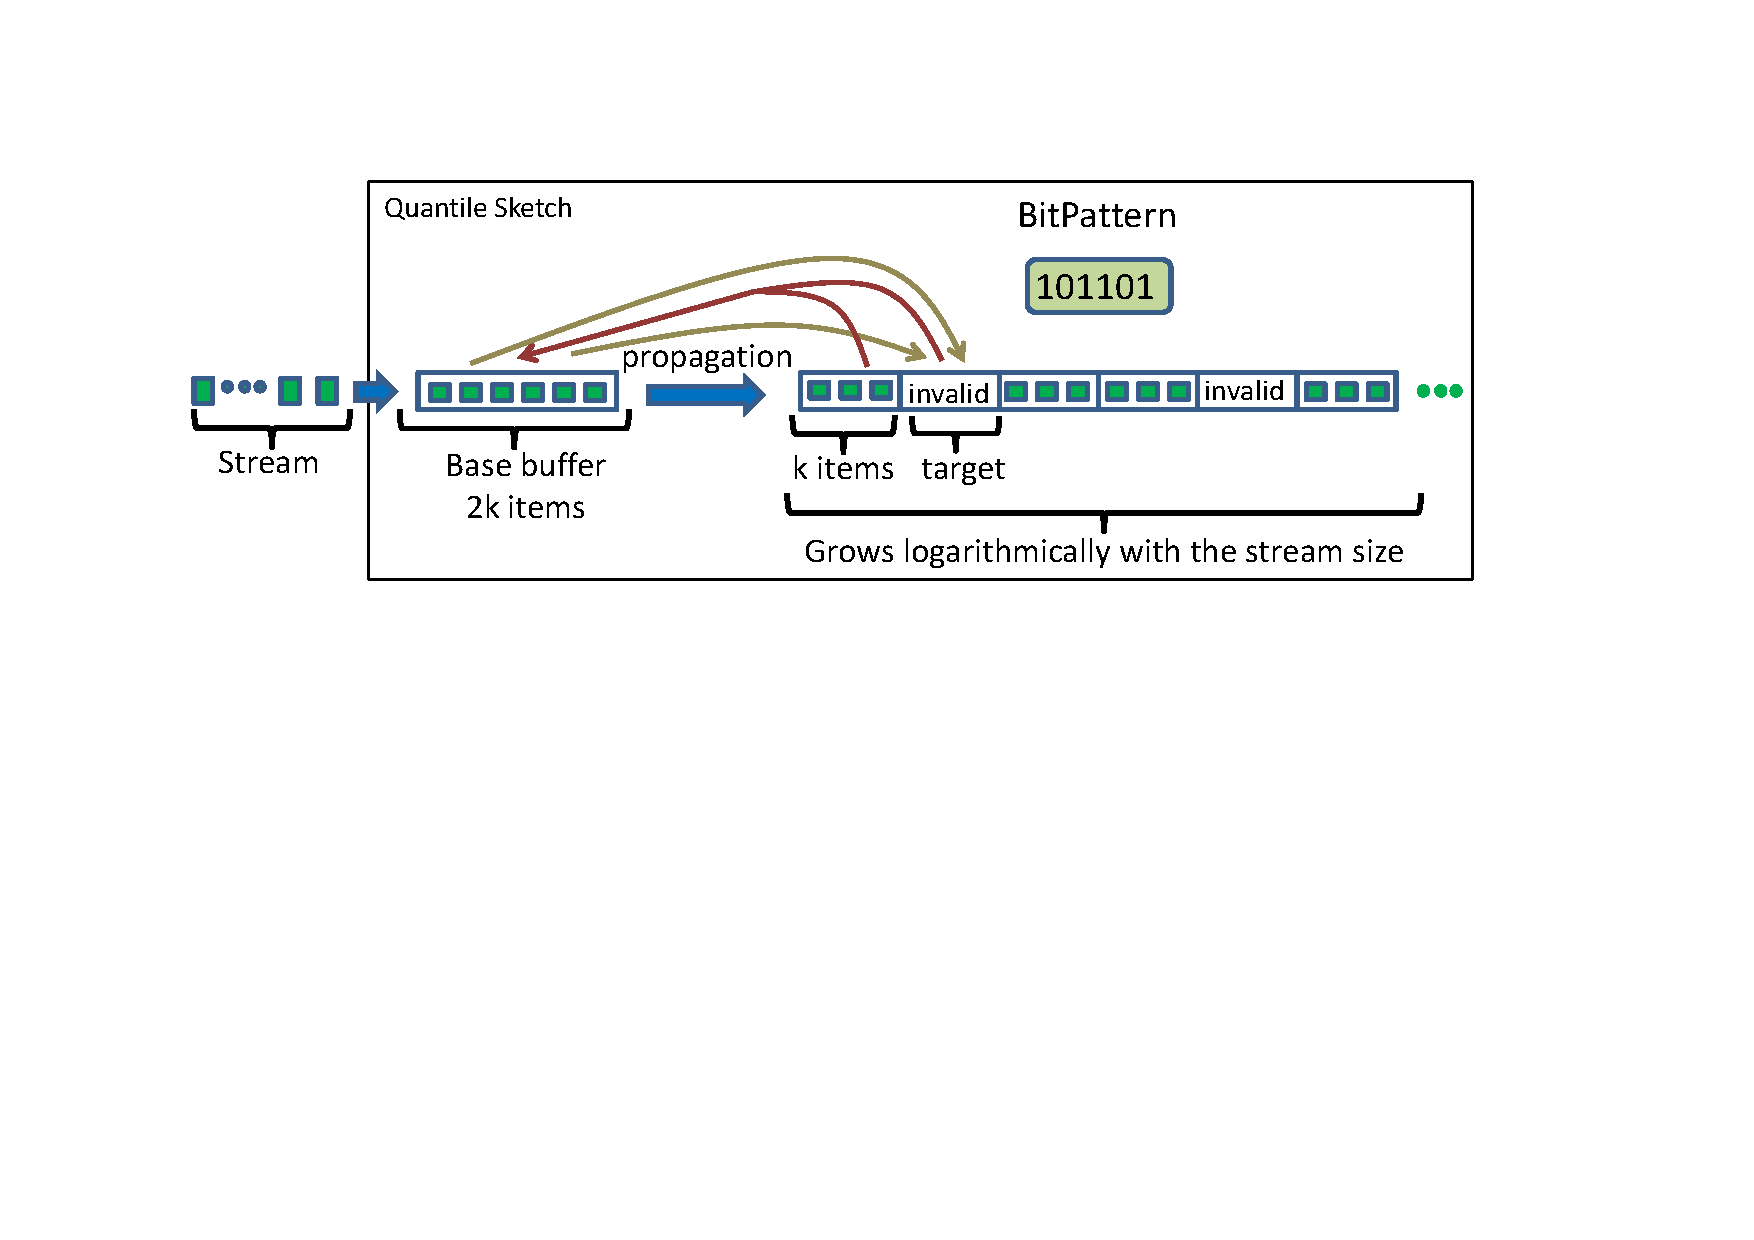
\includegraphics[width=3.2in]{images/quantilesPropogation.pdf}
    \caption{Quantile sketch: Propagating base buffer
    into the levels array.}
    \label{fig:quantilesMerge}
\end{figure}


\subsection{Concurrent Algorithm}

An efficient concurrent algorithm ought to allow  as much work as possible to be executed in parallel.
This is not an easy task since the propagation process (from the base buffer to the levels
array), which takes up most of the work in the algorithm, is
inherently sequential.
Our algorithm decreases the propagation rate without changing
the value of $K$: instead of propagating every $2K$ items we can
do it every $2^{L}K$, where $L \geq 0$ is a parameter that
impacts accuracy. Thus, we amortize the propagation cost and  increase
throughput.

The concurrent quantile algorithm exploits locality and minimizes
synchronization between a single propagation
background thread and many worker threads.
Every worker thread maintains a local sketch with bounded number
of levels; each level stores $b$ items. 
Every time the local sketch fills its last level, 
%and it is the only dataset 1M level 
the content of this  level is propagated to the
shared sketch via the background thread (See Algorithm~\ref{alg:concurrent-quantile}, and Figure~\ref{cocurrentQuntiles}).

\begin{algorithm*}[tb]
\small
\begin{multicols}{2}
\begin{algorithmic}[1]

%\State {\bf Sketch variables:}
\Vars
\State \emph{buf}, init $[ ]$ \Comment global samples
\State \emph{bitPattern}, init 0 \Comment global bit array of valid levels
\Statex
\ForEach{update thread $t_i$}
	\State \emph{q$_i$}, init empty \Comment local quantile sketch
	\State \emph{aux$_i$}, init $[ ]$ \Comment auxiliary array
	\State {\tt atomic} $P_i$, init $1$ \Comment for synchronization
\EndFor
\EndFor

\Statex
\Procedure{query}{$\phi$}
\State \emph{snapshot} $\leftarrow$ \emph{DoubleCollect(buf, bitPattern)}
\ForAll{valid \emph{lvl} in \emph{snapshot.bitPttern}} \label{l:caught-snapshot}
	\ForAll{\emph{sample} in \emph{snapshot.buf[lvl]}}
		\State append $\langle$\emph{sample},\emph{$2^{lvl}$}$\rangle$ to \emph{tuples}
	\EndFor
\EndFor
\State sort $tuples$ by $sample$
\State $pos \leftarrow \min {\{\lfloor N \times \phi \rfloor, N-1\}}$
\State $sum \leftarrow 0$
\State $ind \leftarrow 0$
\While{$sum \leq pos$}
	\State $sum \leftarrow sum + tuples[ind].weight$
	\State $ind \leftarrow ind + 1$
\EndWhile
\State \Return $tuples[ind-1].sample$ 
\EndProcedure
%\Statex

\Procedure{update$_i$}{$val$}
\State insert $val$ into $q_i$
\If{level $L$ in $q_i$ is the single valid full level }
		\State wait until $P_i>0$
		\State $aux_i \leftarrow$ level $L$ in $q_i$
		\State $P_i \leftarrow$ 0
		\State reset $q_i$
\EndIf
\EndProcedure

\Procedure{propagator}{}
\While {true}
\ForAll{update thread $t_i$ s.t. $P_i =0$}
		\State $tmpK \leftarrow aux_i$
		\State $P_i \leftarrow 1$
		\State \emph{target} $\leftarrow$ leftmost zero bit in \emph{bitPattern} $\leq L$
		\State \emph{bitPatternMask} $\leftarrow$ 0
		\For{$i \in \{L,\dots,target-1\}$}
				\State \emph{tmp2K} $\leftarrow$ mergeSort of \emph{tmpK} with \emph{buf[i]}
				\State \emph{tmpK} $\leftarrow$ zip \emph{tmp2K} \label{l:zip}
				\State set bit \emph{i} in \emph{bitPatternMask} to 1
		\EndFor
		\State \emph{buf[target]} $\leftarrow$ \emph{tmpk}
		\State set bit \emph{target} in \emph{bitPatternMask} to 1
		\State \emph{bitPattern} $\Leftarrow$ \emph{bitPattern} $\oplus$ \emph{bitPatternMask}
		\State $N \leftarrow N + K \times 2^{L}$
\EndFor
\EndWhile
\EndProcedure

\end{algorithmic}
\end{multicols}
\caption{Concurrent Quantile sketch algorithm. Maximum level in local sketches is $L$.}
\label{alg:concurrent-quantile}
\end{algorithm*}


The optimal number of local levels depends on the number of
concurrent worker threads.
Since  the propagation time is constant, more worker threads means each thread gets
less help from the background thread; we thus make sure that each thread needs help
less frequently by increasing the number of
local levels. 
%There is a balance point: too much levels means more delay in getting fresh results, not enough levels cause the propagation thread to become a bottleneck.

After triggering propagation to the shared sketch,
a worker thread starts filling its local sketch again.
As in the $\Theta$ sketch, the synchronization between the
propagation thread and  worker thread $t_i$ uses a 
single atomic variable $P_i$.

To propagate level $L$ from a local sketch to the shared sketch,
the propagation thread applies the mechanism of the
sequential quantiles sketch with the following
change:
Instead of starting from zipping the base buffer
into the target level, it starts from level $L$.
If level $L$ in the shared sketch is valid, the propagation
thread merges it (via merge sort) with the local level $L$ into
the base buffer, and continues the propagation to the next level
as before.
The target buffer in this case is the first invalid level that is
not smaller than $L$.
Otherwise, it simply copies the local level $L$ to the shared level
$L$.

Recall that in order to read (getQuantiles), readers build an
auxiliary object based on the levels array and the bitPattern
that describes it.
Therefore, to be able to read concurrently with
background propagation, a reader must obtain a \emph{snapshot} of the
levels array, which is achieved by obtaining 
 a successful  \emph{double collect}~\cite{snapshot}.
The bitPattern is an atomic variable so
that a propagation is visible to all readers after 
it is updated.
To get a snapshot, a reader repeatedly reads the bitPattern, then the levels array,
and then the bitPattern again.
If the bit pattern did not change between the two reads, the
reader has a consistent view.
Otherwise, it tries again.
In parallel, during the propagation process, the background
thread may read many levels, but write only to the target level,
which is invalid at this point.
Therefore, a reader can be sure that the valid levels it reads
between two identical reads of the bitPattern are consistent.
%even though the background thread is propagating in parallel.
%In addition, note that a reader do not have to read all valid
%levels each time it fails to obtain a successful double collect.
%Since a valid level may become invalid and then valid again
%(with different items) only after a higher invalid level becomes
%valid, if two sequential reads of the bitPatern has a
%common suffix, the reader must read only the valid levels in
%the different prefix of the later bitPattern read. 
%It is guaranteed that the valid levels in the suffix are unchanged.

The reads in this algorithm may suffer from starvation due to repeated changes of the bitPattern which prevent the readers from reading a consistent snapshot.
In practice, however, the propagation time (and thus
the time between bitPattern changes) is longer when the target
level is high.
%and every once in a while the background thread must propagate to a high level.
So, eventually the propagation is long enough for
a reader to obtain a snapshot of the levels array. 
The experiments we run show that the readers are 
much faster than the propagator, and the snapshot time is negligible relative to the time it takes to
build the auxiliary object.


\begin{figure}[tb]
    \centering
    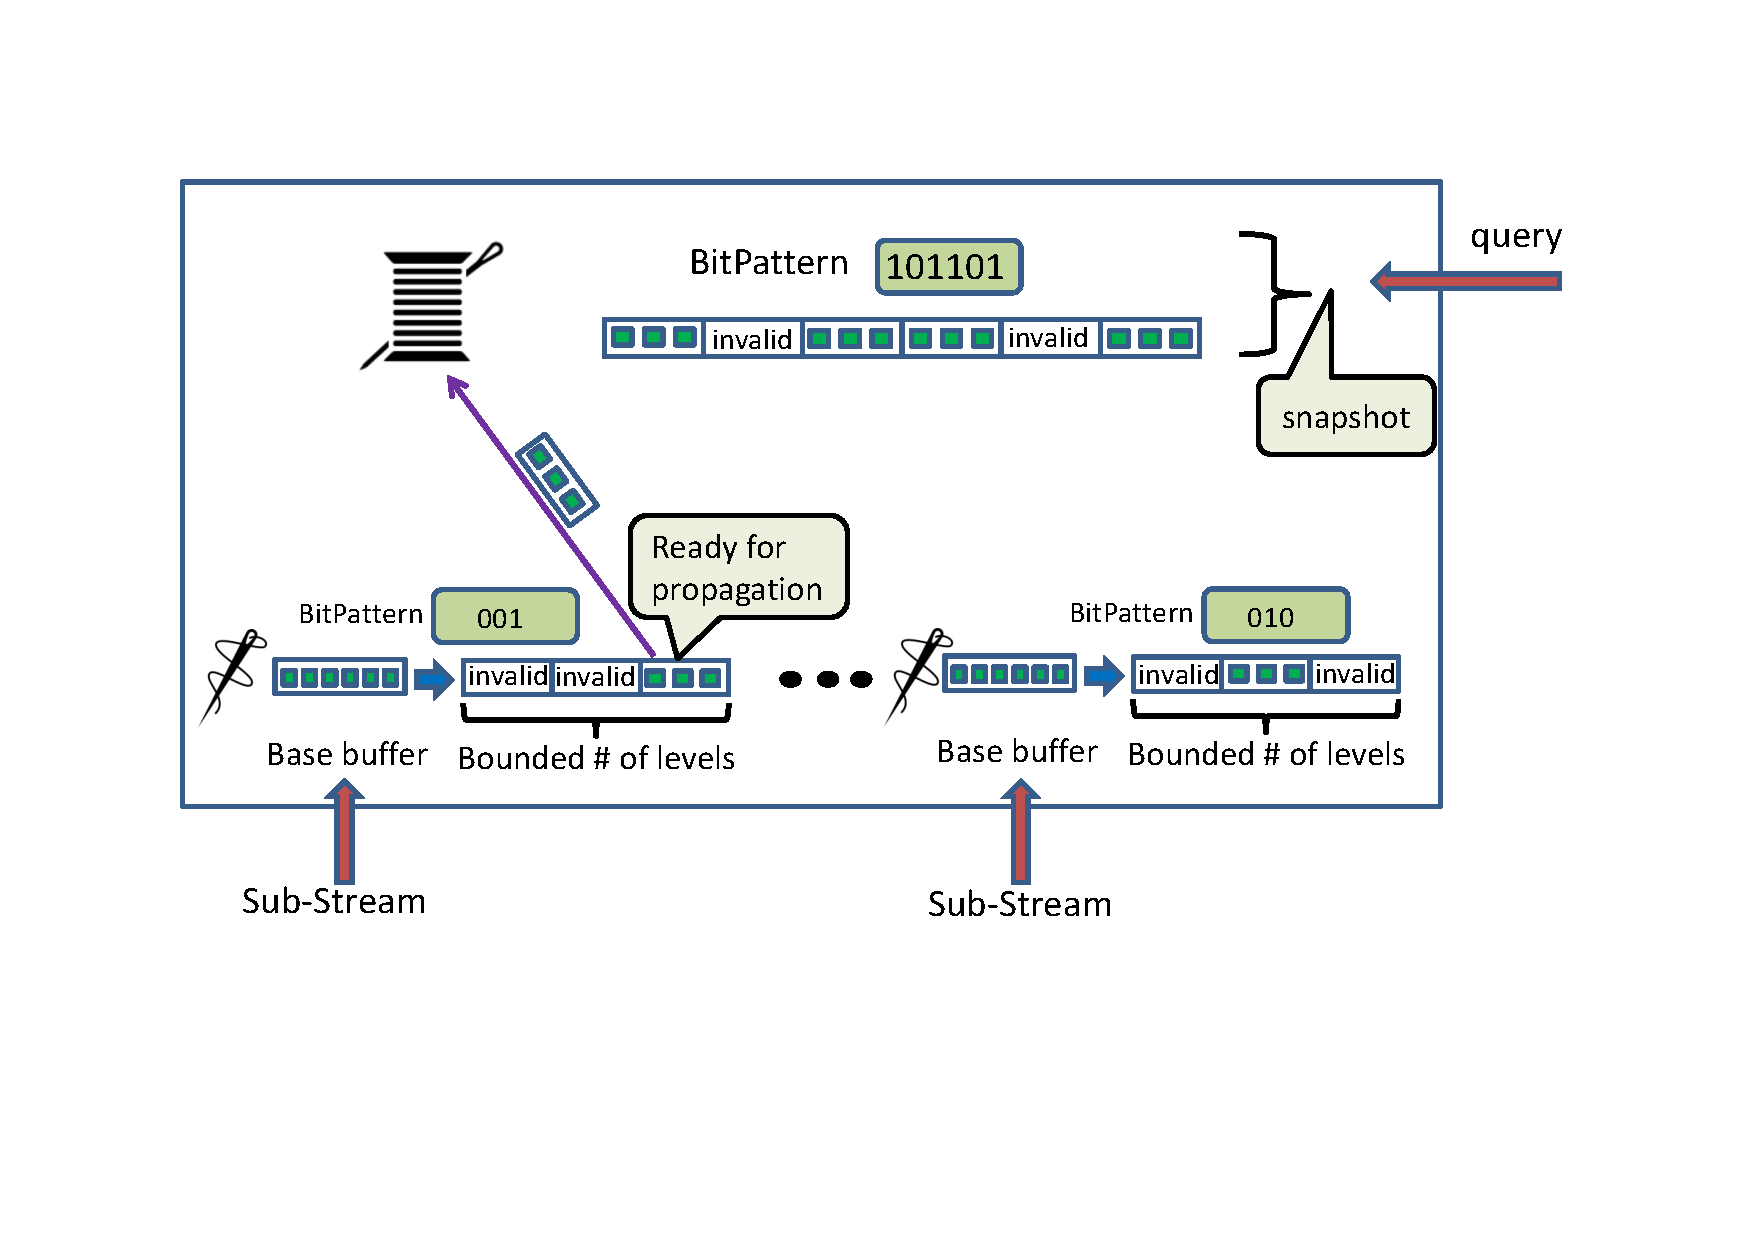
\includegraphics[width=3.5in]{images/cocurrentQuntiles.pdf}
    \caption{Concurrent Quantiles sketch architecture.}
    \label{cocurrentQuntiles}
\end{figure}


%\section{Implementation}
\label{sub:implementation}

We implemented our both concurrent sketches inside
DataSketches~\cite{}, which is a Java open source library
of stochastic streaming algorithms.
In both cases (quantiles and theta), we build our concurrent
sketch on top of the sequential sketch implementation, which was
already very optimized in the library.

To avoid false sharing, unnecessary cash misses, and memory
flashes we let each worker thread to locally maintain its private
part of the sketch.
One way to achieve it is by using thread local memory.
However, since a single sketch update requires so little
computations, we measured that accessing thread local memory per
every operation decreases the update throughput by 30 percent.
Therefore, we choose a different approach that requires little
changes in the API.
Given a shared sketch, instead of calling its methods
directly, every worker thread first wraps it with a context
(sometime called handler) that implements the same interface as
the sketch, and then access the sketch only through its context.
The context is stored private memory that is close to the core
the thread runs on, and it has all the necessary information
(e.g., thread id) that the worker thread has to know in order to 
work with the shared sketch.  



%Code example?


\section{Evaluation}
\label{sec:evaluation}




We implement our concurrent sketches and evaluate its
performance.
Our implementation for both concurrent sketches is based on the
algorithms implemented in DataSketches~\cite{}, which is a Java
open source library of stochastic streaming algorithms.
%We implemented our both concurrent sketches inside
%DataSketches~\cite{}, which is a Java open source library
%of stochastic streaming algorithms.
In both cases (quantiles and theta), we build our concurrent
sketch on top of the sequential sketch implementation, which was
already very optimized in the library.

In Section~\ref{sub:imp} we give some of the implementation
details.
In Section~\ref{sub:setup} we describe the experiment setup.
In Section~\ref{sub:thetaExp} we compare our Concurrent Theta
sketch with the sequential implementation given in
DataSketches library, and in Section~\ref{sub:quantilesExp} we do
it for the quantiles sketch. 


\subsection{Implementation}
\label{sub:imp}

To avoid false sharing, unnecessary cash misses, and memory
flashes we let each worker thread to locally maintain its private
part of the sketch.
One way to achieve this is by using thread local memory.
However, since a single sketch update requires so little
computations, we measure that accessing thread local memory per
every operation decreases the update throughput by 30 percent.
Therefore, we choose a different approach that requires little
changes in the API.
Given a shared sketch, instead of calling its methods
directly, every worker thread first wraps it with a context
(sometime called handler) that implements the same interface as
the sketch, and then access the sketch only through its context.
The context is stored the memory that is close to the core
the thread runs on, and it has all the necessary information
(e.g., thread id) that the worker thread has to know in order to 
work with the shared sketch.

  

\subsection{Experiment Setup}
\label{sub:setup}

The experiments were run on a dedicated machine with four Intel
Xeon E5-4650 processors, each with $8$ cores, for a total of
$32$ threads (with hyper-threading disabled).
For the experiments we use microbenchmarks, and consider two
representative workloads: (1) an \emph{update-only} workload in
which a sketch is built from a stream, and (2) a \emph{mixed}
workload in which there is a single reader that continuously read
from the sketch, while the other threads build it.
We run every experiment for 30 seconds. 
Our baselines are the the sketches' sequential implementations
given in the DataSketches library that we wraped with a read/write lock
to allow concurrency.

\subsection{Theta sketch}
\label{sub:thetaExp}

Since we are not familiar with prior works on concurrent Theta
and quantiles sketches, our only baseline is the very optimized
sequential implementation given in DataSketches that we wrap with
a read/write lock.
As we mention before, the cost of acquiring a lock in every
operation on the sketch is very high since the sketches are
inherently very fast data structures.
Figure~\ref{fig:LockIsBadTheta} compares the throughput of the
sequential implementation Theta sketch given in DataSketch with
ans without a lock.

\begin{figure}[t!]
    \centering
    \begin{subfigure}[t]{0.49\textwidth}
        \centering
        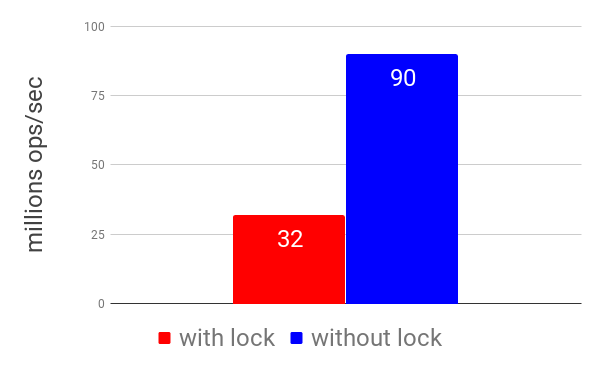
\includegraphics[width=3.2in]{images/seqTheta}
        \caption{}
        \label{fig:LockIsBadTheta}
    \end{subfigure}%
    ~ 
    \begin{subfigure}[t]{0.49\textwidth}
        \centering
        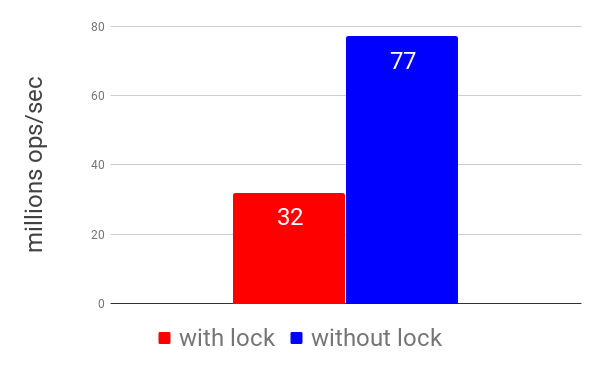
\includegraphics[width=3.2in]{images/seqQuantiles}
        \caption{}
        \label{fig:LockIsBadQuantiles}
    \end{subfigure}
    \caption{}
    \label{fig:sequntial}
\end{figure}

In Figure~\ref{fig:ConccurentTheta} we compare the scalability
between our concurrent sketch and the original sketch wrapped
with a read/write lock in a update only workload.
As expected, the lock based sequential sketch does not scale, and
in fact it performs worse when accessed concurrently by many
threads.
However, our sketch achieves almost perfect scalability.
In this graph we show results with the following parameters:
Every local buffer contains 16 items, while the size of the
shared sketch is 4096 items.
We run each experiment for 30 seconds.
It is important to note the we also tried smaller local buffers,
and shorter runs and the results were the same.

\begin{figure}[h]
  \centering
  \includegraphics*[width=4in]{images/concurrentThetaGraph}
  \caption{}
   \label{fig:ConccurentTheta}
\end{figure}




In Figure~\ref{fig:ConccurentThetaReads} we compare the
throughput of the reader, between
our concurrent sketch and the original sketch wrapped with a
read/write lock, in a mix workload.
We also measured the updates throughput in the present of one
reader, but we omit this graph since it looks exactly the same as
the one in Figure~\ref{fig:ConccurentTheta}.
We can see that in our sketch the reader is able to read 380
millions time in a second independtly of the number of concurrent
writers, while sequential lock-based's sketch is able to support
only 0.2 millions per second in case of one conccurent writer,
and it goes down to 0.0006 millions reads per seocnd when the
number of writers grows to 28.
We achieve stable very high throughput because the reader in our
sketch simply read one atomic variable, which does not
interfere the background thread, while in the sequential
lock-based's sketch the reader pay the fence price in addition
to competing with all the writers on acquiring the lock.  



\begin{figure}[h]
  \centering
  \includegraphics*[width=4in]{images/concurrentThetaReads}
  \caption{}
   \label{fig:ConccurentThetaReads}
\end{figure}




\subsection{Quantiles sketch}
\label{sub:quantilesExp}

As for the Theta sketch, our only baseline here is a very
optimized sequential implementation given in the DataSketch
library.
Figure~\ref{fig:LockIsBadQuantiles} shows that as in the Theta
case, wrapping the sequential quantiles sketch with a read/write
lock decreases throughput by almost a factor of 3 even with a
single thread.

In Figure~\ref{fig:ConccurentQuantilesUpdate} we compare the
throughput of our Quantiles sketch to the baseline.
First, note that the baseline does not scale, and moreover, it
achieves best result with a single worker thread.
Our sketch, on the contrary, scale perfectly when every thread
has enough local levels.
It clearly follows from the graph that in order for the
background thread to support more worker threads we have to
increase the number local levels.
O local levels are enough for 2 threads, 2 local levels are good
for 12 threads, and for perfect scalability on our machine in
update-only workload we need 4 local levels.


%we can shoe also the partition result and talk about locality.
% 1. the prcie of fences
% 2. the price of bringing new sketche to local memory and pay
% the cash missess.

\begin{figure}[h]
  \centering
  \includegraphics*[width=4in]{images/QuantilesUpdate}
  \caption{}
   \label{fig:ConccurentQuantilesUpdate}
\end{figure}

In Figure~\ref{fig:ConccurentQuantilesReader} we consider a
mixed workload to check how a single reader impact the update
throughput.
Since the reader in this case continuously reads the atomic
bitPattern variable, and thus forces the background thread to
flash its local memory more often, we see that the background
thread indeed works harder.
Instead of 4 levels in the update-only workload, we now need 5
local levels for perfect scalability, and we can also see that
0 and 2 local levels allow the background thread to support less
worker threads than in the update-only workload.




\begin{figure}[h]
  \centering
  \includegraphics*[width=4in]{images/QuantilesMixed}
  \caption{}
   \label{fig:ConccurentQuantilesReader}
\end{figure}


\section{Discussion}
\label{sec:discussion}

We present a general approach for implementing concurrent data sketches. Specifically, we describe concurrent algorithms and implementations for the Theta and Quantile sketches. We measure the performance of these sketches and show they scale almost linearly with the number of sketch, out-performing their sequential and lock-based counterparts. We are currently in the process of committing this code to the DataSketch library. In the future we plan to integrate it with applications like Druid by replacing the lock-based instantiation  and to measure the affect on ingestion and query performance in real-time indexing.            


 %
\section{Introduction}

%\subsection{Motivation and goals}

% stream processing for RT analytics
Real-time analytics are becoming increasingly prevalent in many businesses. 
Examples include Yahoo's Flurry~\cite{flurry},  
%\footnote{\url{https://developer.yahoo.com/flurry/docs/analytics/}},
the technology behind Mobile Developer Analytics, and Digits Yahoo Corporate-Wide dashboard for monitoring KPIs and traffic trends%at different granularities
~\cite{digits},
%\footnote{\url{https://digits3.yahoo.com}},
as well as Google's F1~\cite{Shute2013}, which powers its AdWords
%\footnote{\url{https://www.google.com/adwords/}}
business.
Such systems need to process massive data streams and answer queries about them in real-time.
% examples
A common query, for example, is estimating the number of \emph{unique elements} in a long stream, which 
can be used to count how many different users access a particular web page or application. 
A second example is a \emph{quantiles} estimator, which can be used, for example, to  answer questions like  \emph{what percentage of user sessions end within one minute?} or \emph{what is the median session time?}

% Sketches
In order to serve such queries, analytics engines use 
\emph{data sketches}, or \emph{sketches} for short. A sketch is essentially 
a succinct summary of a long stream. 
Sketches are built in a single pass over the stream via sampling or by applying a filter 
that retains a small subset  of the stream elements. 
%They are designed to take up a small memory footprint, since analytics engines 
%often keep tens or hundreds of thousands and sometimes even millions of 
%sketches in memory~\cite{Druid}.
% Sketches are fast
Due to the massive scale of the incoming data,   library functions producing sketches
are optimized to be extremely fast, often digesting millions of stream elements per second~\cite{sketchesLibrary}. 

%For example, the $\Theta$ sketch in the Java Sketches Library \inred{add reference} 
%estimates the number of unique elements in a stream; it can process millions of stream 
%elements a second. 

 % Missing: r-w concurrency 
 Analytics engines need to answer real-time queries while  stream data continues to flow in.
 One way this is done 
today is by building sketches in epochs, and querying the sketch only after
 the epoch ends. An alternative approach is using locks to prevent concurrent access to a sketch.
 For example, in the Java Sketches Library~\cite{sketchesLibrary},  an 
attempt to query a sketch  while it is being updated  may encounter an inconsistent
intermediate state, leading to a gross estimation error. Therefore, applications like Druid~\cite{druid}
currently use sketches conservatively within a \emph{synchronized} block.
% and queries directed to a sketch must wait  for its construction to complete. 
Our first goal in this paper is to eliminate such waiting, and to allow queries to proceed 
concurrently with stream updates. 

% MIssing: w-w concurrency
In addition to the required concurrency among queries and updates,
it is also desirable to allow
concurrency among update threads in order to expedite the sketch building process on multi-core platforms. 
The common approach today is to build separate sketches from substreams, 
and then merge them via a dedicated union operation~\cite{multi-KMV}. 
In this approach, queries cannot be served before the final union completes. 
Our second goal is therefore to allow multiple threads to update a common, 
queryable sketch. The challenge is to do so without slowing down the update threads,
given that access to shared data requires  synchronization via costly memory fences 
and shared data updates can cause frequent invalidations in L1 caches, severely impacting performance. 
Figure~\ref{fig:lockBased} compares the throughput of two 
%  the
sequential sketch implementations given in DataSketch with
and without a lock. We see that 
the cost of acquiring a lock  is  high, since  sketches are
inherently fast structures.

\begin{figure}[t!]
    \centering
    \begin{subfigure}[t]{0.49\columnwidth}
        \centering
        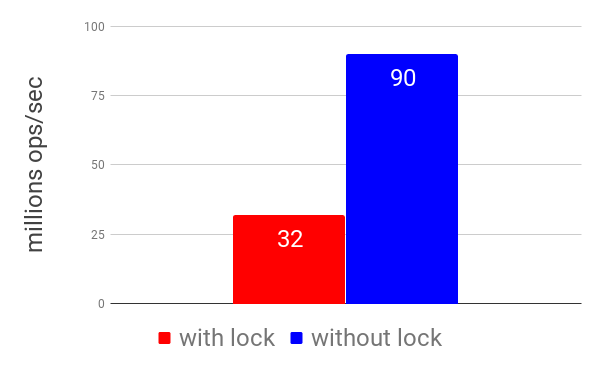
\includegraphics[width=1.6in]{images/seqTheta}
        \caption{Theta sketch}
        \label{fig:LockIsBadTheta}
    \end{subfigure}%
    ~ 
    \begin{subfigure}[t]{0.49\columnwidth}
        \centering
        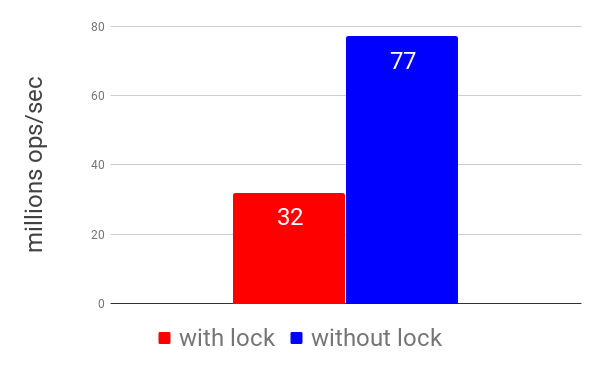
\includegraphics[width=1.6in]{images/seqQuantiles}
        \caption{Quantile sketch}
        \label{fig:LockIsBadQuantiles}
    \end{subfigure}
    \caption{Throughput of sequential sketch vs. lock-based sketch running a single write-only thread.}
    \label{fig:lockBased}
\end{figure}



% This paper
In this paper 
we present a general approach for building concurrent sketches that
constantly reflect all data processed by multiple update threads, 
and serve queries at any time. % during the stream processing. 
 % Basic idea for parallelizing
Our  approach employs multiple worker threads that buffer sketches of bounded-size substreams in thread-local memory, while a dedicated helper thread 
periodically \emph{propagates} these local buffers into a shared data structure via a union-like operation.
 Reducing data contention and the frequency of synchronization between the worker threads and the propagator is instrumental for achieving good performance. Queries are served from the shared data structure, and are carefully 
 designed to take its \emph{consistent snapshot} in case it is updated in parallel with them.

We implement our approach for two popular sketches in the Java Sketches Library -- Theta~\cite{Theta},
which estimates the number of unique elements in a stream, and quantiles~\cite{quantiles}.
%worst-case error an adversarial scheduler can induce, 
Experiments show the algorithms scales almost linearly: with 28 threads, update throughput is an order of magnitude greater than with a single threads, while the 
read throughput is 3 orders of magnitude greater than that of a lock-based implementation.  


 
 
 % \section{Model}
\label{sec:model}




\subsection{Streaming}


We consider a problem of a single sketch summary that is built
from infinite streams of data items such that there is a
dedicated thread to every stream that only it processes.
We denote by $S_{e,p}$ a sketch that with probability $p$
returns answer with an error of at most $e$ in respect to the
items that have been processed, and we denote by $n(t)$ the
number of items that were processed (by all threads) by time
$t$.

\subsection{Relaxed semantics}





% In order to define concurrent correct behavior we need first to
% define how the sketch should behave in sequential runs.
% The sequential specification of a sketch $S_{e,p}$ is the
% following:
% For all times $t$, every query that
% completes at $t$ returns an answer with an error of at most $e$
% in respect to $n(t)$.

Since data items arrive in streams, and each stream can
potentially have multiple sources in the real world and some
links in the network my be faster than others, it follows
that (1) the order in which events appear in a stream is not
necessarily the order in which they were generated and (2) some
of the items can be lost in the way.
In addition, since sketches are inherently approximate and all
updates commute, providing solutions with linearizabilty in
respect to strict semantics is an overkill.
It makes more sense, to provide a slightly weaker safety
guarantee that allows reads (statistical quires) to miss some of
the processed data items if we can exploit it to provide
more efficient solutions.

In this paper we consider a semantic relaxation that we believe
makes a lot of sense in sketches.
Our relaxation is a variation of an out-of-order relaxation
presented in~\cite{Henzinger}, which in turn generalized the
relaxation presented in~\cite{Afek}.

Intuitively, we allow every read (statistical quire) to miss
a bounded number of updates that precedes it.
Formally, given a sequential specification of some sketch
$sk$, we define the \emph{k-perforated sequential specification}
of $sk$ in the following way:
A sequential run $r$ of $sk$ satisfies $sk$'s \emph{perforated
specification} if for every read $rd$ in $r$ there is run $r'$
that is identical to $r$ except of at most $k$ updates
that appear in $r$ and not in $r'$, in which $rd$ satisfies
$sk$'s sequential specification.

Given a concurrent run $r$ of a sketch $sk$, we say that a
\emph{k-perforated linearization} $L_r$ of $r$ is a
sequential run that satisfies $r$'s operation precedence
relation and $sk$'s \emph{k-perforated sequential specification}.
We say that a concurrent sketch $sk$ is \emph{k-perforated
relaxation} if every run of $sk$ has a \emph{k-perforated
linearization}.


\subsection{General Scheme}
\label{sub:generalScheme}




Given a sketch $sk$ with a sequential implementation $S$ such
that every run of $S$ satisfies $sk$'s sequential specification,
we give a general scheme to create a concurrent version of
$S$ that satisfies \emph{k-perforated linearization}.
First, extend $S$ to support concurrent reads, and denote this
implementation by $S'$.
Then, a generic structure that includes (1) a shared
instance of $S'$; and (2) local data structures $L_1,.. L_n$
that buffer operations to be added to $S'$.
To satisfy \emph{k-perforated linearization} ensure that ($A_1$)
all buffer contain no more than k operations together; and
($A_2$) the propagation from each $L_i$ to $S'$ is equivalent to
running the sequence of operations masked by $L_i$ on $S'$.
In the following sections we present two concurrent algorithms
using the above structure and prove that they satisfy conditions
$A_1$ and $A_2$.


    
 % \input{sections/dynamicStorage.tex}
 % \input{sections/circumventImpossibility.tex}
 % \input{sections/summaryAndFutureWork.tex}
 % \appendix
 % \input{sections/appendixProofAlg.tex}

%\newpage
\bibliographystyle{plain}
%\bibliographystyle{splncs03}
\bibliography{sketches}




%\newpage


\end{document}
